%Please make sure to set your compiler to XeLaTeX to compile this document properly

\documentclass[12pt]{article}
\usepackage{setspace}
\onehalfspacing
\setstretch{1.5}
\usepackage{graphicx}
\usepackage{enumerate}
\usepackage{enumitem}
\usepackage{sectsty}
\usepackage{xcolor}
\usepackage{fontspec}
\usepackage[backend=biber, style=ieee]{biblatex} % Use biblatex
\usepackage{subcaption}
\usepackage{fancyhdr}
\usepackage{pgfplots}
\pgfplotsset{compat=1.18}
\usepackage{setspace}


%Replace the LOGOS.png file with your own logo here. 
\newcommand{\mylogo}{\includegraphics[width=5cm]{LOGOS.png}}

\AtBeginBibliography{\small}
\definecolor{navy}{rgb}{0,0,0.5} % RGB values for navy, other high contrast colours can work too.

\setmainfont{OpenDyslexic} %This is an accessible font, if you want to support the developers work or access the font for your own projects, you can donate here: https://opendyslexic.org/

\pagecolor{yellow!10} %The colours chosen here are high contrast and are easier for people with visual impairments such as colourblindness to read. 
\color{navy}

% Adjust page margins
\usepackage{geometry}
\geometry{
    left=2cm,    % Adjust the left margin as needed
    right=2cm,   % Adjust the right margin as needed
    top=2cm,     % Adjust the top margin as needed
    bottom=2cm,  % Adjust the bottom margin as needed
}

% Left-align the text, justified is not suitable for people who are dyslexic, struggle with tracking, etc.
\raggedright

\setlength{\parskip}{10pt}

\addbibresource{Bib.bib} % Set your bibliography file


\begin{document}

\begin{titlepage}
\centering
\mylogo % Your logo or image
\vspace{2cm}

\Huge Accessible Template for Research Papers\\[1ex]
\large This version uses the IEEE citation style \\
\vspace{1cm}
\large C Kelly \\
\end{titlepage}



\begin{abstract}
This is where you can write your abstract for your paper. Lorum Ipsum etc. 

This template was designed to be accessible for a number of disabilities. When sending this to people, make sure to double check that you have the reading order set correctly. For more information on how to do this go to https://etc.usf.edu/techease/4all/web-accessibility/changing-the-reading-order-of-a-pdf-document-with-adobe-acrobat/
\end{abstract}

\section{Introduction}
\pagestyle{plain}
This is your first section. "The introduction typically describes the scope of the document and gives a brief explanation or a summary of the document. It may also explain certain elements that are important to the document. The readers can thus have an idea about the following text before they actually start reading it" \cite{wikipedia-contributors-2023}. And that is a placeholder citation.

\newpage %use this command to move the content following it to a new page

\section{This is a New Section}


\subsection{And this is a Subsection, with figures and lists}

The way that this template is laid out, it should be relatively straightforward to copy your pre-existing LaTeX files into it. 

This is a list!
\begin{itemize}
  \item Item 1
  \item Item 2,
  \item Item 3,
  \item Item 4,
  \item etc.
\end{itemize}

\begin{figure}[htbp]
  \centering
  \includegraphics[width=0.3\linewidth]{TestImage.jpg} %you can adjust the size of your figure, just change the width or switch to a \width=5cm or \textwidth command instead. 
  \caption{This is a sample figure!}
  \label{fig}
\end{figure}



\newpage
\section{Graphs and Tables}

\subsection{Table}
\begin{table}[htbp]
  \centering
   \renewcommand{\arraystretch}{1.5}
  \caption{My Sample Table}
  \begin{tabular}{|c|c|c|}
    \hline
    \textbf{Header 1} & \textbf{Header 2} & \textbf{Header 3} \\
    \hline
    Row 1, Col 1 & Row 1, Col 2 & Row 1, Col 3 \\
    Row 2, Col 1 & Row 2, Col 2 & Row 2, Col 3 \\
    \hline
  \end{tabular}
\end{table}

\subsection{Graph}

\begin{figure}[htbp]
  \centering
  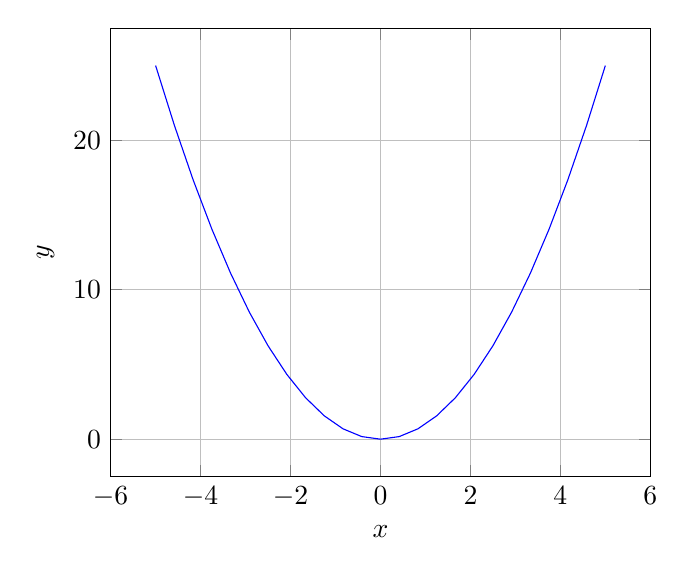
\begin{tikzpicture}
    \begin{axis}[
      xlabel={$x$},
      ylabel={$y$},
      grid=both,
      ]
      \addplot[blue,mark=none] {x^2};
    \end{axis}
  \end{tikzpicture}
  \caption{A Simple Plot}
\end{figure}


 \footnote{\textit{This is a footnote!}}

\printbibliography
\end{document}
